% \begin{frame}{\tciv{} \dqnes{}}
%     \onslide<2->{
%     \begin{figure}
%     \centering
%     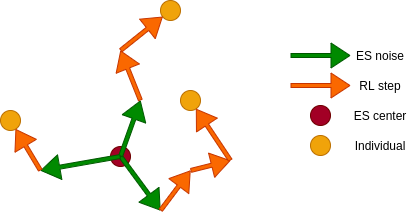
\includegraphics[width=.7\linewidth]{images/DQNES/scheduled.drawio.png}
%     \caption{Distribution of weight values in networks evolved with different encodings.}
%     \end{figure}
%     }
% \end{frame}

\begin{frame}{\tciv{} Using samples to drive the search}%
    \begin{figure}


    \tikzset{every picture/.style={line width=0.75pt}} %set default line width to 0.75pt        

    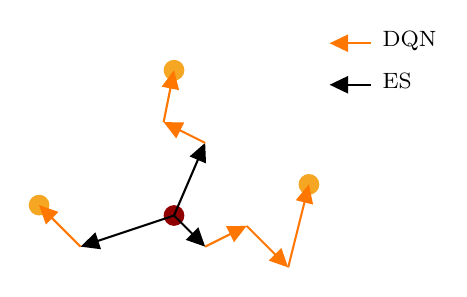
\begin{tikzpicture}[x=0.75pt,y=0.75pt,yscale=-1,xscale=1]
    %uncomment if require: \path (0,300); %set diagram left start at 0, and has height of 300
        % Center
        \onslide<2->{
        %Flowchart: Connector [id:dp7892172092869572] 
        \draw  [draw opacity=0][fill={rgb, 255:red, 145; green, 0; blue, 0 }  ,fill opacity=1 ] (270,155) .. controls (270,152.24) and (272.24,150) .. (275,150) .. controls (277.76,150) and (280,152.24) .. (280,155) .. controls (280,157.76) and (277.76,160) .. (275,160) .. controls (272.24,160) and (270,157.76) .. (270,155) -- cycle ;
        }

        % End points
        \onslide<4->{
        %Flowchart: Connector [id:dp8059049646076628] 
        \draw  [draw opacity=0][fill={rgb, 255:red, 245; green, 166; blue, 35 }  ,fill opacity=1 ] (205,150) .. controls (205,147.24) and (207.24,145) .. (210,145) .. controls (212.76,145) and (215,147.24) .. (215,150) .. controls (215,152.76) and (212.76,155) .. (210,155) .. controls (207.24,155) and (205,152.76) .. (205,150) -- cycle ;
        %Flowchart: Connector [id:dp5011381675096028] 
        \draw  [draw opacity=0][fill={rgb, 255:red, 245; green, 166; blue, 35 }  ,fill opacity=1 ] (270,85) .. controls (270,82.24) and (272.24,80) .. (275,80) .. controls (277.76,80) and (280,82.24) .. (280,85) .. controls (280,87.76) and (277.76,90) .. (275,90) .. controls (272.24,90) and (270,87.76) .. (270,85) -- cycle ;
        %Flowchart: Connector [id:dp3773909027910184] 
        \draw  [draw opacity=0][fill={rgb, 255:red, 245; green, 166; blue, 35 }  ,fill opacity=1 ] (335,140) .. controls (335,137.24) and (337.24,135) .. (340,135) .. controls (342.76,135) and (345,137.24) .. (345,140) .. controls (345,142.76) and (342.76,145) .. (340,145) .. controls (337.24,145) and (335,142.76) .. (335,140) -- cycle ;
        }

        \onslide<3->{
        %Straight Lines [id:da6809885341795275] 
        \draw    (275,155) -- (232.85,169.05) ;
        \draw [shift={(230,170)}, rotate = 341.57] [fill={rgb, 255:red, 0; green, 0; blue, 0 }  ][line width=0.08]  [draw opacity=0] (8.93,-4.29) -- (0,0) -- (8.93,4.29) -- cycle    ;
        %Straight Lines [id:da34929359178134534] 
        \draw    (275,155) -- (288.82,122.76) ;
        \draw [shift={(290,120)}, rotate = 113.2] [fill={rgb, 255:red, 0; green, 0; blue, 0 }  ][line width=0.08]  [draw opacity=0] (8.93,-4.29) -- (0,0) -- (8.93,4.29) -- cycle    ;
        %Straight Lines [id:da4067586836296815] 
        \draw    (275,155) -- (287.88,167.88) ;
        \draw [shift={(290,170)}, rotate = 225] [fill={rgb, 255:red, 0; green, 0; blue, 0 }  ][line width=0.08]  [draw opacity=0] (8.93,-4.29) -- (0,0) -- (8.93,4.29) -- cycle    ;
        %Straight Lines [id:da7752837053635281] 
        \draw    (370,92) -- (353,92) ;
        \draw [shift={(350,92)}, rotate = 360] [fill={rgb, 255:red, 0; green, 0; blue, 0 }  ][line width=0.08]  [draw opacity=0] (8.93,-4.29) -- (0,0) -- (8.93,4.29) -- cycle    ;
        % Text Node
        \draw (374,85) node [anchor=north west][inner sep=0.75pt]  [font=\footnotesize] [align=left] {ES};
        }

        \onslide<4->{
        %Straight Lines [id:da5651183383226251] 
        \draw [color={rgb, 255:red, 255; green, 118; blue, 0 }  ,draw opacity=1 ]   (230,170) -- (212.12,152.12) ;
        \draw [shift={(210,150)}, rotate = 45] [fill={rgb, 255:red, 255; green, 118; blue, 0 }  ,fill opacity=1 ][line width=0.08]  [draw opacity=0] (8.93,-4.29) -- (0,0) -- (8.93,4.29) -- cycle    ;
        %Straight Lines [id:da9174794629852384] 
        \draw [color={rgb, 255:red, 255; green, 118; blue, 0 }  ,draw opacity=1 ]   (290,170) -- (307.32,161.34) ;
        \draw [shift={(310,160)}, rotate = 153.43] [fill={rgb, 255:red, 255; green, 118; blue, 0 }  ,fill opacity=1 ][line width=0.08]  [draw opacity=0] (8.93,-4.29) -- (0,0) -- (8.93,4.29) -- cycle    ;
        %Straight Lines [id:da9236788570029154] 
        \draw [color={rgb, 255:red, 255; green, 118; blue, 0 }  ,draw opacity=1 ]   (310,160) -- (327.88,177.88) ;
        \draw [shift={(330,180)}, rotate = 225] [fill={rgb, 255:red, 255; green, 118; blue, 0 }  ,fill opacity=1 ][line width=0.08]  [draw opacity=0] (8.93,-4.29) -- (0,0) -- (8.93,4.29) -- cycle    ;
        %Straight Lines [id:da5363883614541579] 
        \draw [color={rgb, 255:red, 255; green, 118; blue, 0 }  ,draw opacity=1 ]   (330,180) -- (339.27,142.91) ;
        \draw [shift={(340,140)}, rotate = 104.04] [fill={rgb, 255:red, 255; green, 118; blue, 0 }  ,fill opacity=1 ][line width=0.08]  [draw opacity=0] (8.93,-4.29) -- (0,0) -- (8.93,4.29) -- cycle    ;
        %Straight Lines [id:da8537813572490652] 
        \draw [color={rgb, 255:red, 255; green, 118; blue, 0 }  ,draw opacity=1 ]   (290,120) -- (272.68,111.34) ;
        \draw [shift={(270,110)}, rotate = 26.57] [fill={rgb, 255:red, 255; green, 118; blue, 0 }  ,fill opacity=1 ][line width=0.08]  [draw opacity=0] (8.93,-4.29) -- (0,0) -- (8.93,4.29) -- cycle    ;
        %Straight Lines [id:da4405746369803901] 
        \draw [color={rgb, 255:red, 255; green, 118; blue, 0 }  ,draw opacity=1 ]   (270,110) -- (274.41,87.94) ;
        \draw [shift={(275,85)}, rotate = 101.31] [fill={rgb, 255:red, 255; green, 118; blue, 0 }  ,fill opacity=1 ][line width=0.08]  [draw opacity=0] (8.93,-4.29) -- (0,0) -- (8.93,4.29) -- cycle    ;
        %Straight Lines [id:da8366023954327625] 
        \draw [color={rgb, 255:red, 255; green, 118; blue, 0 }  ,draw opacity=1 ]   (370,72) -- (353,72) ;
        \draw [shift={(350,72)}, rotate = 360] [fill={rgb, 255:red, 255; green, 118; blue, 0 }  ,fill opacity=1 ][line width=0.08]  [draw opacity=0] (8.93,-4.29) -- (0,0) -- (8.93,4.29) -- cycle    ;
        
        % Text Node
        \draw (374,65) node [anchor=north west][inner sep=0.75pt]  [font=\footnotesize] [align=left] {DQN};
        }

\end{tikzpicture}

    \end{figure}
\end{frame}